

\documentclass[conference]{IEEEtran}
%\usepackage {makecell}
\usepackage {url}
\usepackage {graphicx}
%\usepackage {caption}
\usepackage {algorithm}
\usepackage {algorithmic}
%\usepackage {algpseudocode}
\usepackage{amsmath}
\usepackage{tabu}
\usepackage[numbers,sort&compress]{natbib}
\usepackage{bbding}
% correct bad hyphenation here
\hyphenation{op-tical net-works semi-conduc-tor}

\begin{document}
% paper title
\title{Joint Energy-Aware and Buffer-Assisted Relay Selection Method for Relay-Aided D2D Communications}

% author names and affiliations
% use a multiple column layout for up to three different
% affiliations
\author{\IEEEauthorblockN{Lei Yu\IEEEauthorrefmark{1}, Xiaoxiang Wang\IEEEauthorrefmark{1}, Dongyu Wang\IEEEauthorrefmark{1}\Envelope}
\IEEEauthorblockA{\IEEEauthorrefmark{1}
 Key Lab. of Universal Wireless Comm., Ministry of Education, \\
 Beijing Univ. of Posts and Telecom., \\
 Beijing, P.R. China\\
Email(s): \{zzmikkz, cpwang, dy\_wang\}@bupt.edu.cn}}


% make the title area
\maketitle
% As a general rule, do not put math, special symbols or citations
% in the abstract
\begin{abstract}
Device--device (D2D) communication is a effective technique to improve performance on overall throughput and energy efficiency in cellular network. However, owing to the long separation distances or poor link quality between the source and destination user devices (UDs), the advantages of D2D communications is limited by only using direct D2D communication. For enhancing traffic capacity in cellular network, relay-aided D2D communications was put forward as a complement to direct D2D communications. The purpose of this article is to devise a relay selection method that improve the D2D communication performance. In this paper, we propose an Energy-Aware and Buffer-Assisted (EABA) relay selection method that take account of certain conditions jointly, including transmission rate, relay-available UD (RUD) residual energy, and RUD buffer state. At each time slot, according to the channel states, energy, and buffer size, a scheduling rule is calculated dynamically by the EABA relay selection method. And then, which of the source or relay nodes is activated to transmit packet is specified by the scheduling rule. Simulation results confirm the performance of the proposed method about the file transmission time and the total amount of data transmitted under RUD residual energy and RUD buffer state.
\\
\textbf {\small \emph{Keywords --- Device-to-device communication, Relay selection, Limited energy, Buffer-Aided}}
\end{abstract}

\IEEEpeerreviewmaketitle
\section{Introduction}
% no \IEEEPARstart
To satisfy the increasing demand of mobile communication, device-to-device (D2D) communications is proposed as a effective technique for cellular network \cite{5350367,7949342,7254241}. D2D communication includes licensed-band D2D and unlicensed-band D2D \cite{7128330}. Unlicensed-band D2D communication is usually exposed to uncontrolled interference. Therefore, most works in this field study in licensed-band D2D communications, in order to improve the overall cellular network performance, such as spectrum and energy efficiency, by using mode selection and frequency reuse \cite{7878672,7504380,7742334}.

However, a majority of recent works have only studied direct D2D (one-hop D2D) communications. The advantages of D2D communications is limited by only using direct D2D communication, because the failure of direct D2D communications is probably caused by the long separation distances or poor link quality between the source and destination D2D-capable user devices (DUDs) \cite{7876267}. To solve the question, relay-aided D2D communications, which works in the way that two DUDs within an BS's coverage communicate with each other, with the help of a relay under BS's control \cite{7450161,7752964}, was supposed to explore the benefits of D2D communications. The range of D2D communications can be obviously extended by using relay \cite{7925800}.

Compared to fixed relay \cite{6775376}, the relay-capable UD (RUD) aided D2D communications may be more helpful owing to the increase of UD density. Thus,  most of the works used RUD instead of fixed relay in relay-aided D2D Communications. With the help of a RUD,  two DUDs be able to communicate with each other even if the long separation distances or poor link quality between them \cite{7450161,7752964}.


To apply relay-aided D2D communications in cellular network, the most important work is to select optimal RUD for each DUD communication pair under BS's control. The issues of Relay selection have been widely discussed in cellular network cooperative communications. Most relay selection strategies are executed in two successive time slots, where at the previous slot, the packets are sent from source to relay and at the next slot, the destination receive the data transmitted by the relay. This relaying method is known as conventional relaying \cite{6807959}. Moreover, most of the existing relay selection methods focused on physical layer (PHY), the residual energy and buffer state of candidate relay node was basically ignored. What's more, the channel reuse is not included in  most of these methods.

In this paper, we focused on relay-aided D2D communication which be known as a complement to direct D2D communication in cellular network. Besides, both direct and relay-aided D2D communication should reuse the wireless resources of general cellular user devices (CUDs). According to the channel state of each link, RUD residual energy and RUD buffer state, a joint  Energy-Aware and Buffer-assisted (EABA) relay selection method which calculates the weight of each link at each time slot is presented in this paper. Then, the method selects the link with the highest priority to transmit data instead of conventional relaying \cite{7562509}.

The rest of this paper is organized as follows. We introduce a system model for relay-assisted D2D communications in cellular network and formulates optimization problems in Section \uppercase\expandafter{\romannumeral2}. A joint Energy-Aware and Buffer-Aided (EABA) relay selection method is proposed in Section \uppercase\expandafter{\romannumeral3}. The simulation results and analysis are presented in Section \uppercase\expandafter{\romannumeral4}, followed by the conclusions in Section \uppercase\expandafter{\romannumeral5}.

\section{System Model and Problem Formulation}
As shown in Fig. 1, we study at a scenario that composed of CUDs, RUDs, DUDs, all of which are controlled by BS. We assume that there is only one source and destination DUD in the cellular. We also assume that there are $M$ CUDs which communicate with the BS through cell uplink channels and $N$ idle user devices which can be used as RUDs. In the following sections, we let $C_{1},C_{2},\ldots,C_{i},\ldots,C_{M}$ denote $M$ CUDs, and $R_{1},R_{2},\ldots,R_{j},\ldots,R_{N}$ denote $N$ RUDs, i.e., $i\in\left[1,2,\ldots,M\right]$ and $j\in\left[1,2,\ldots,N\right]$. The source DUD is denoted by $S$ and the destination DUD is denoted by $D$.
%Fig1
\begin{figure}[!t]
\center
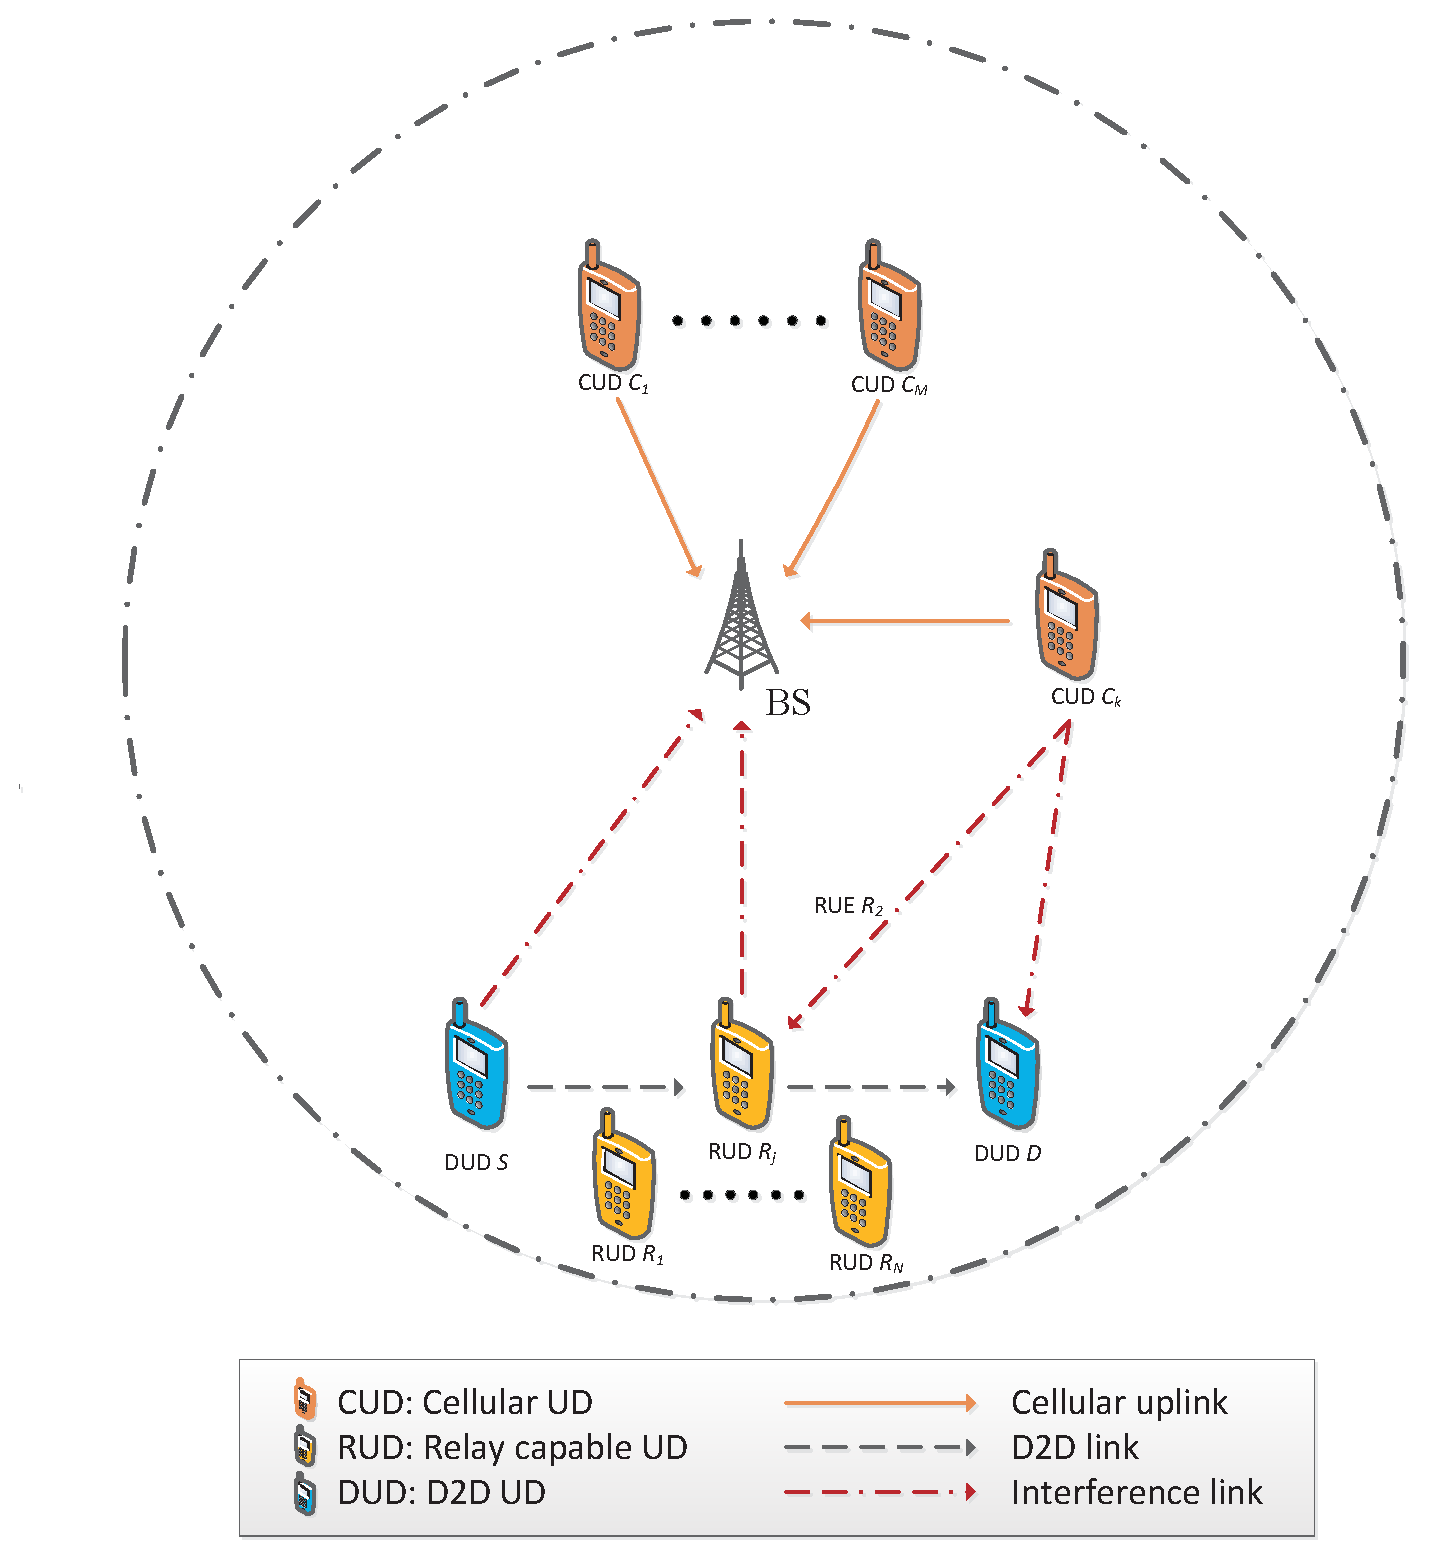
\includegraphics[width=3.5in]{fig1}
%where an .eps filename suffix will be assumed under latex,
% and a .pdf suffix will be assumed for pdflatex; or what has been declared
% via \DeclareGraphicsExtensions.
\caption{A D2D communications system model underlaying cellular network, in which D2D communication reuses the uplink frequency of CUD $C_k$. DUDs $S$ denote the source D2D UDs and DUDs $D$ denote the destination D2D UDs. RUD $R_j$ is the selected relay UD for relay-aided D2D communications.}
\label{fig_success}
\end{figure}

Moreover, presume that $M$ CUDs use $M$ separated cell uplink channels which have same bandwidth and can be reused by D2D communication. Based on these assumptions, we only consider the interference from the reused CUDs to the RUD and the $D$ and the interference from the $S$ and RUD to the BS.

In addition, assumed that the BS can acquire the channel state information(CSI) of all links and that the D2D mode, RUD and reuse uplink selection is decided by the BS. Besides, we assume that both CUDs uplink channels and D2D links should meet the minimum of SINR requirement.

The channel model which consider path loss, slow fading and fast fading can be expressed as \cite{6560489}:
\begin{equation}
|{h_{s,d}}|^{2} = K_{0}\beta_{s,d}\zeta_{s,d}\cdot L_{s,d}^{-\alpha}
\end{equation}
|{h_{s,d}}|^{2} is the channel gain between two UDs or between a UD and the BS. $K_{0}$ is a constant determined by cellular parameters. $\beta_{s,d}$ and $\zeta_{s,d}$ denote slow and fast fading gains with log-normally and exponential distribution, respectively. $\alpha$ is the path loss exponent and $L_{s,d}$ is the distance between $s$ and $d$

The purpose of this paper is to efficiently utilize cellular frequency resources, RUD residual energy and RUD buffer state to minimize transmission time and maximize total amount of data transmitted, before the communication between the source and the destination  becomes unavailable. Let $T\left(\chi\right)$ represent the file transmission time of method $\chi$, in other words, the transmission time since the first packet is transmitted by the $S$ until the last packet is received by the $D$, the problem can be expressed as
\begin{align}
&\displaystyle \min _{\mathcal {\chi}} ~T(\mathcal {\chi})
\\[-5pt]&\text {subject to} ~ \sum T_{j} \leq \tau_j(1) , \quad \forall j , \tag{2a}
\\[-1.5pt]&\qquad \qquad ~ j\in\left[1,2,\ldots,N\right] , \tag{2b}
\end{align}
where $\sum T_{j}$ denote RUD $R_{j}$ total working time, $N$ denote the total number of packets, and $ \tau_j(1)$ denote the residual work time of relay $R_j$ in time slot 1.

\section{EABA Relay Selection Method}
As discussed above, an optimal link should be selected by the BS according to transmission rate, RUD residual energy and RUD buffer state. Hence, in this section, we demonstrate the methods of estimation of the transmission rates of the links between DUDs and RUDs, the residual energies and buffer states of RUDs. We will also propose a relay selection method to address the problem in Section \uppercase\expandafter{\romannumeral2}.

\subsection{Link Data Rate Estimation}
As shown in Fig. 1, the link data rate is derived in this subsection. Let $P_{C_i},P_S$, and $P_{R_j}$ represent the transmit power of the CUD $C_i$, the source DUD, and RUD $R_j$, respectively. In addition, we suppose that the noise $n_0$ at each receiver UD is additive white Gaussian noise (AWGN) drawn from a zero-mean normal distribution with variance $\sigma^2$, i.e., $n_0 \sim (0,\sigma^2)$. RUD $R_j$ is assumed to work on half-duplex mode. If link $S \rightarrow R_j$ is selected as a transmission link and the uplink channel of $C_i$ $(i \in [1,2,\ldots,M])$ is selected as the reuse channel, the received signal at $R_j$ can be expressed as
\begin{equation}
y^i_{S,R_j} = h_{S,R_j}\cdot x_S + h_{C_i,R_j}\cdot x_{C_i} + n_0
\end{equation}
where $x_S$ is the signal transmitted from the $S$, $h_{C_i,R_j}\cdot x_{C_i}$ denote the interference from CUD $C_i$ to $R_j$. If link $R_j \rightarrow D$ is selected as a transmission link and the uplink channel of $C_k$ $(k \in [1,2,\ldots,M])$ is reused, the received signal at destination DUD $D$ can be expressed as
\begin{equation}
y^k_{R_j,D} = h_{R_j,D}\cdot x_{R_j} + h_{C_k,D}\cdot x_{C_k} + n_0
\end{equation}
where $x_S$ is the signal transmitted from $R_j$, $h_{C_k,D}\cdot x_{C_k}$ denote the interference from CUD $C_k$ to $D$.

The SINR of $R_j$ and the $D$ are
\begin{equation}
\gamma^{i}_{S,R_j} = \frac{P_S|{h_{S,R_j}}|^{2}}{P_{C_i}|{h_{C_i,R_j}}|^{2} + \sigma^2} ,\gamma^{k}_{R_j,D} = \frac{P_{R_j}|{h_{R_j,D}}|^{2}}{P_{C_k}|{h_{C_k,D}}|^{2} + \sigma^2}
\end{equation}
respectively. The achievable data rate of link $S \rightarrow R_j$ and $R_j \rightarrow D$ can be expressed as
\begin{equation}
R_{S,R_j} = B\log_2(1 + \gamma^{i}_{S,R_{j}}),R_{R_j,D} = B\log_2(1 + \gamma^{k}_{R_j,D})
\end{equation}
respectively, where $B$ denote the channel bandwidth.

Likewise, the SINR of BS is
\begin{equation}
\gamma^{j}_{C_i,B} = \frac{P_{C_i}|{h_{C_i,B}}|^{2}}{P_S|{h_{S,B}}|^{2} + \sigma^2} ,\gamma^{j}_{C_k,B} = \frac{P_{C_k}|{h_{C_k,D}}|^{2}}{P_{R_j}|{h_{R_j,B}}|^{2} + \sigma^2}
\end{equation}
respectively, where B in this equation denote BS.

\subsection{RUD Residual Energy And Buffer State Estimation}
Owing to the limited energy of the relay, each relay can forward a limited amount of data before the energy is exhausted. Thus, even though a relay has sufficient buffer size, it's no use sending more data to the relay than it can forward later. To take this into account, we should know the data size can be transmitted of RUD $R_i$ under the residual energy.

Let $E_{1},E_{2},\ldots,E_{j},\ldots,E_{N}$ denote the total energies of $N$ RUDs, respectively. To describes the influences of the discharge current and transmission power of each RUD on RUD remaining work time, Peukert's Law \cite{6981957} is expressed as
\begin{equation}
\tau_j = E_j/I^{\alpha}_j
\end{equation}
where $\tau_j$ is the remaining work time of $R_j$, $I_j$ is discharge current, and $\alpha$ is the Peukert constant and its usually equal to 1.3 \cite{6981957}. Using $P_{R_j}$ denotes the transmission power of $R_j$, the discharge current can be expressed as
\begin{equation}
$I_j = P_{R_j} / V_0$
\end{equation}
where $V_0$ denote the discharge voltage of each UD and predefine the same $V_0$ for each UDs.

Therefore, we can establish the remaining work time of each RUD which we know residual energy, transmission power, and discharge voltage. In this paper, the transmission power of all UDs are predefined as a fixed value, so we can use the remaining operation time $\tau_j$ denotes the residual energy of RUD $R_j$. Then the minimum data size can be transmitted of RUD $R_j$ can be expressed as
\begin{equation}
\theta_j = R_{min} \cdot \tau_j
\end{equation}
where $R_{min}$ is the minimum transmission speed of RUD $R_j$
%Fig2
\begin{figure}[!t]
\center
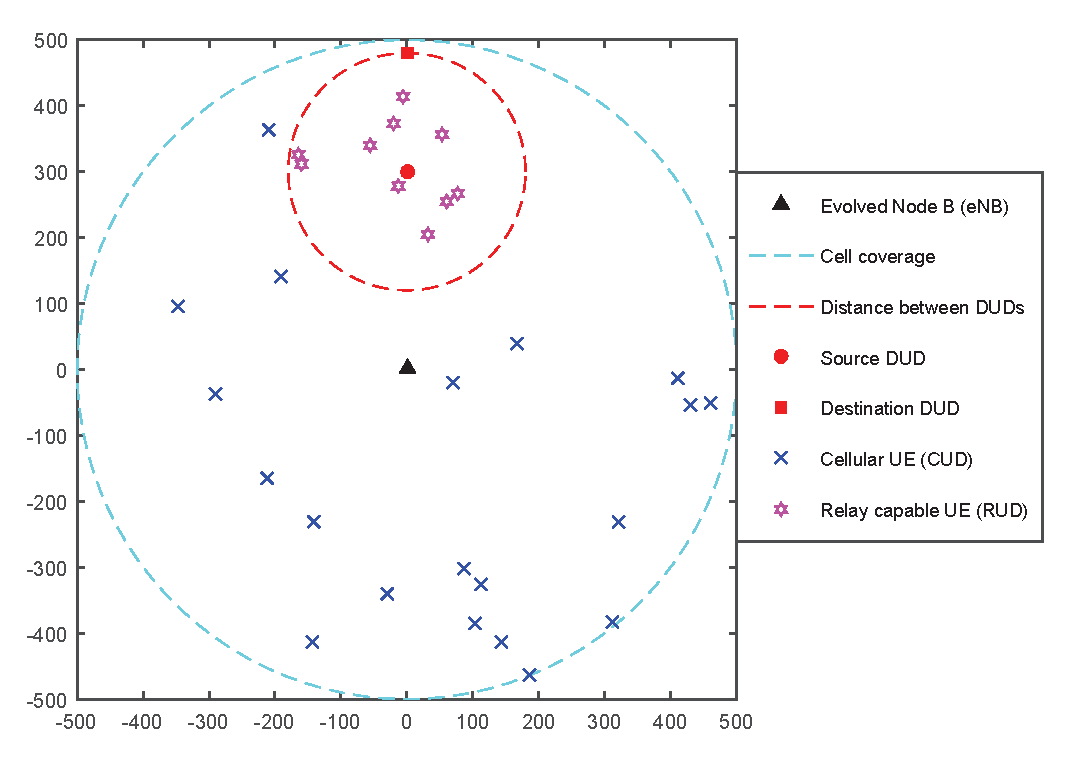
\includegraphics[width=3.5in]{fig2}
%where an .eps filename suffix will be assumed under latex,
% and a .pdf suffix will be assumed for pdflatex; or what has been declared
% via \DeclareGraphicsExtensions.
\caption{The simulation of the scenario. The distance between the $S$ and $D$ is 220m.}
\label{fig_scenario}
\end{figure}

Moreover, we specify a time slot is a unit duration, and the residual energy of the relay which is selected to transmit data is decreased by its transmission time, e.g., $\tau_j(t+1) = \tau_j(t) - tran_j(t)$, where $tran_j(t)$ denotes the transmission time of RUD $R_j$ to the destination. $Q_j(t)$ is the amount of data stored in the buffer of RUD $R_j$ at the starting of time slot $t$, and $e_j(t) = L_j -  Q_j(t)$, where $L_j$ denotes the total buffer size of RUD $R_j$, so $e_j(t)$ is the buffer size of RUD $R_j$ can be used at the starting of time slot $t$. And then, the $tran_j(t)$ can be expressed as
\begin{equation}
tran_j(t) = \begin{cases}T & R_{R_j,D}(t)\cdot T \leq Q_j(t)\\Q_j(t)/R_{R_j,D}(t) & R_{R_j,D}(t)\cdot T > Q_j(t)\end{cases}
\end{equation}
where $T$ is duration of a time slot, and $R_{R_j,D}(t)$ is the data rate of link $R_j \rightarrow D$ at time slot $t$.

\subsection{EABA Strategy}
For the purpose of transmitting the file as quickly as possibly, Energy-Aware and Buffer-Assisted (EABA) executes depending on the following theory: the relay which has a log of residual energy and buffer space should  have a higher priority to recept data. On the other hand, if the relay has a large number of data in its buffer, it should get a higher priority to transmit data to the destination. What's more, a link with a high SNIR, more data will be transmitted at a time slot, should have a higher chance to transmit data.

In the EABA method, the BS calculates the weight of every link $S \rightarrow R_j$ as
\begin{equation}
W_{S\rightarrow R_j} = min(\theta_j - Q_j,e_j) \cdot R_{S\rightarrow R_j} \cdot I[\gamma_{S\rightarrow R_j} \geq \gamma_d)]
\end{equation}
while $I[x]$ is a deictic function, which is zero if x is false and one otherwise. Hence, a link $S \rightarrow R_j$ get a positive weight only if relay $R_j$ has enough buffer space and residual energy, and the link SINR must no less than the predefined SINR requirement for D2D link.

Similarly, for link $R_j \rightarrow D$, the BS calculates the weight as
\begin{equation}
W_{R_j \rightarrow D} = Q_j \cdot R_{R_j \rightarrow D} \cdot I[\gamma_{R_j \rightarrow D} \geq \gamma_d)]
\end{equation}
According to (12), a link $R_j \rightarrow D$ get a valid weight only when relay $R_j$ has data stored in its buffer, and the link SINR must not less than the predefined SINR requirement for D2D link.

After adopting EABA method calculating the weight, the link $l_max$ which has the highest weight is selected, where
\begin{equation}
l_max = \arg \max_{l \in \{S \rightarrow R_j\} \cup \{R_j \rightarrow D\}}\{W_l\}
\end{equation}

\begin{algorithm}[!t]
\caption{EABA Relay Selection Method}
\begin{algorithmic} [1]
\STATE {Each relay computes the minimum data size can be transmitted using (9) and sends residual energy and buffer state to the BS.}
\STATE{The BS computes the weight for link $S \rightarrow R_j$ using (11).}
\STATE{The BS computes the weight for link $S \rightarrow R_j$ using (12).}
\STATE {Under BS control, the best link is selected based on (13).}
\end{algorithmic}
\end{algorithm}

Algorithm 1 shows the execution process of the EABA method. The EABA method considers transmission rate of each link, residual energy and buffer state of each relay, so the BS needs to know all of there information. When the link with the highest weight is activated by BS, the BS will notify the whole D2D network either the $S$ should transmit to the selected relay or the selected relay  transmit to the $D$.

As long as the network is available, the procedure of EABA continues. Depending on the above discussion of the EABA method, if relay $R_j$ has data stored in its buffer, $R_j$ will have enough energy to transmit that data. Note that there will be a time slot in which that link $R_j \rightarrow D$ will have a good channel condition, $R_j$ will transmit the data which has been stored in $R_j$ to the $D$ successfully. Hence, if the network becomes unavailable, there will be no data stored in relay $R_j$.

\section{Simulation Results}
In this section, we provide simulations in MATLAB to evaluate the proposed relay selection method. Simulation is performed in a single cellular, and we assume that the cellular radius is 500 meters. We also assume that all CUDs are random distributed in the cellular. Besides, there are only two DUDs (the $S$ and the $D$), and all RUDs are random distributed in  a circular area with the distance between the $S$ and the $D$ as its radius and the $S$ as its center. The simulation of the scenario is shown in Fig. 2, and Table \uppercase\expandafter{\romannumeral1} lists main parameters used in this paper. Since all UDs are re-deployed random in different test, we did 100,000 times experiments at the same scenario for getting an average result.

%Table 1
\begin{table}[!t]
  \centering
  \scriptsize
  \caption{Simulation parameters}
  \label{tab:notations}
  \begin{tabular}{m{3cm}m{3cm}}
    \\[-2mm]
    \hline\\[-2mm]
    {\bf  Parameters}& {\bf Value}\\
    \hline
    \hline
    \vspace{1mm}\\[-3mm]
    Cellular radius      &    500 m\\
    \hline
    \vspace{1mm}\\[-3mm]
    Noise density &    -174 dBm/Hz \\
    \hline
    \vspace{1mm}\\[-3mm]
    UE transmit power  &  24 dBm\\
    \hline
    \vspace{1mm}\\[-3mm]
    The number of CUD  &  20 \\
    \hline
    \vspace{1mm}\\[-3mm]
    The number of DUD  &  10 \\
    \hline
    \vspace{1mm}\\[-3mm]
    Path loss exponent ($\alpha$) &  4 \\
    \hline
    \vspace{1mm}\\[-3mm]
    Path loss constant ($K_0$) &   0.01\\
    \hline
    \vspace{1mm}\\[-3mm]
    SINR requirements ($\gamma_c,\gamma_d$) &  20 dB \\
    \hline
    \vspace{1mm}\\[-3mm]
    Slow fading coefficient ($\beta_{a,b}$) &  Log-normal distribution with mean value of zero and standard deviation of 10 dB\\
    \hline
    \vspace{1mm}\\[-3mm]
    Fast fading coefficient ($\zeta_{a,b}$) &  Exponential distribution with unit mean\\
    \hline
    \vspace{1mm}\\[-3mm]
    Number of packet in source DUE &  50 \\
    \hline
    \vspace{1mm}\\[-3mm]
    packet size &  1024 bits\\
    \hline
    \vspace{1mm}\\[-3mm]
    A unit time slot ($\triangle T$) &  $1 \mu s$\\
    \hline
    \vspace{1mm}\\[-3mm]
    RUE total energy ($E_i$) &  Randomly distributed in [0,1440] mAh \\
    \hline
  \end{tabular}
\end{table}

The proposed relay selection method, considering transmission rate, RUD residual energy and RUD buffer state, is validated by the simulations as shown in Fig. 3, 4, 5. To evaluate the necessity of the proposed relay selection method, we make a comparison of "EABA relay selection" with "random relay selection" and "rate based relay selection". All the three relay selection methods assume that direct D2D mode is unavailable, that is to say, the three methods are only working in relay-Aided D2D mode. Moreover, we also ignore the time and energy consumption caused by calculation. In "random relay selection", the BS will select a link randomly from link $S\rightarrow R_j$ and link $R_j\rightarrow D$; in "rate based relay selection", the BS will select a link has maximum SINR, i.e., the maximum transmission rate, from link $S\rightarrow R_j$ and $R_j\rightarrow D$; while in the "EABA relay selection", the BS will select the optimal link calculated by the formula which is proposed in Section \uppercase\expandafter{\romannumeral3}.

%Fig3
\begin{figure}[!t]
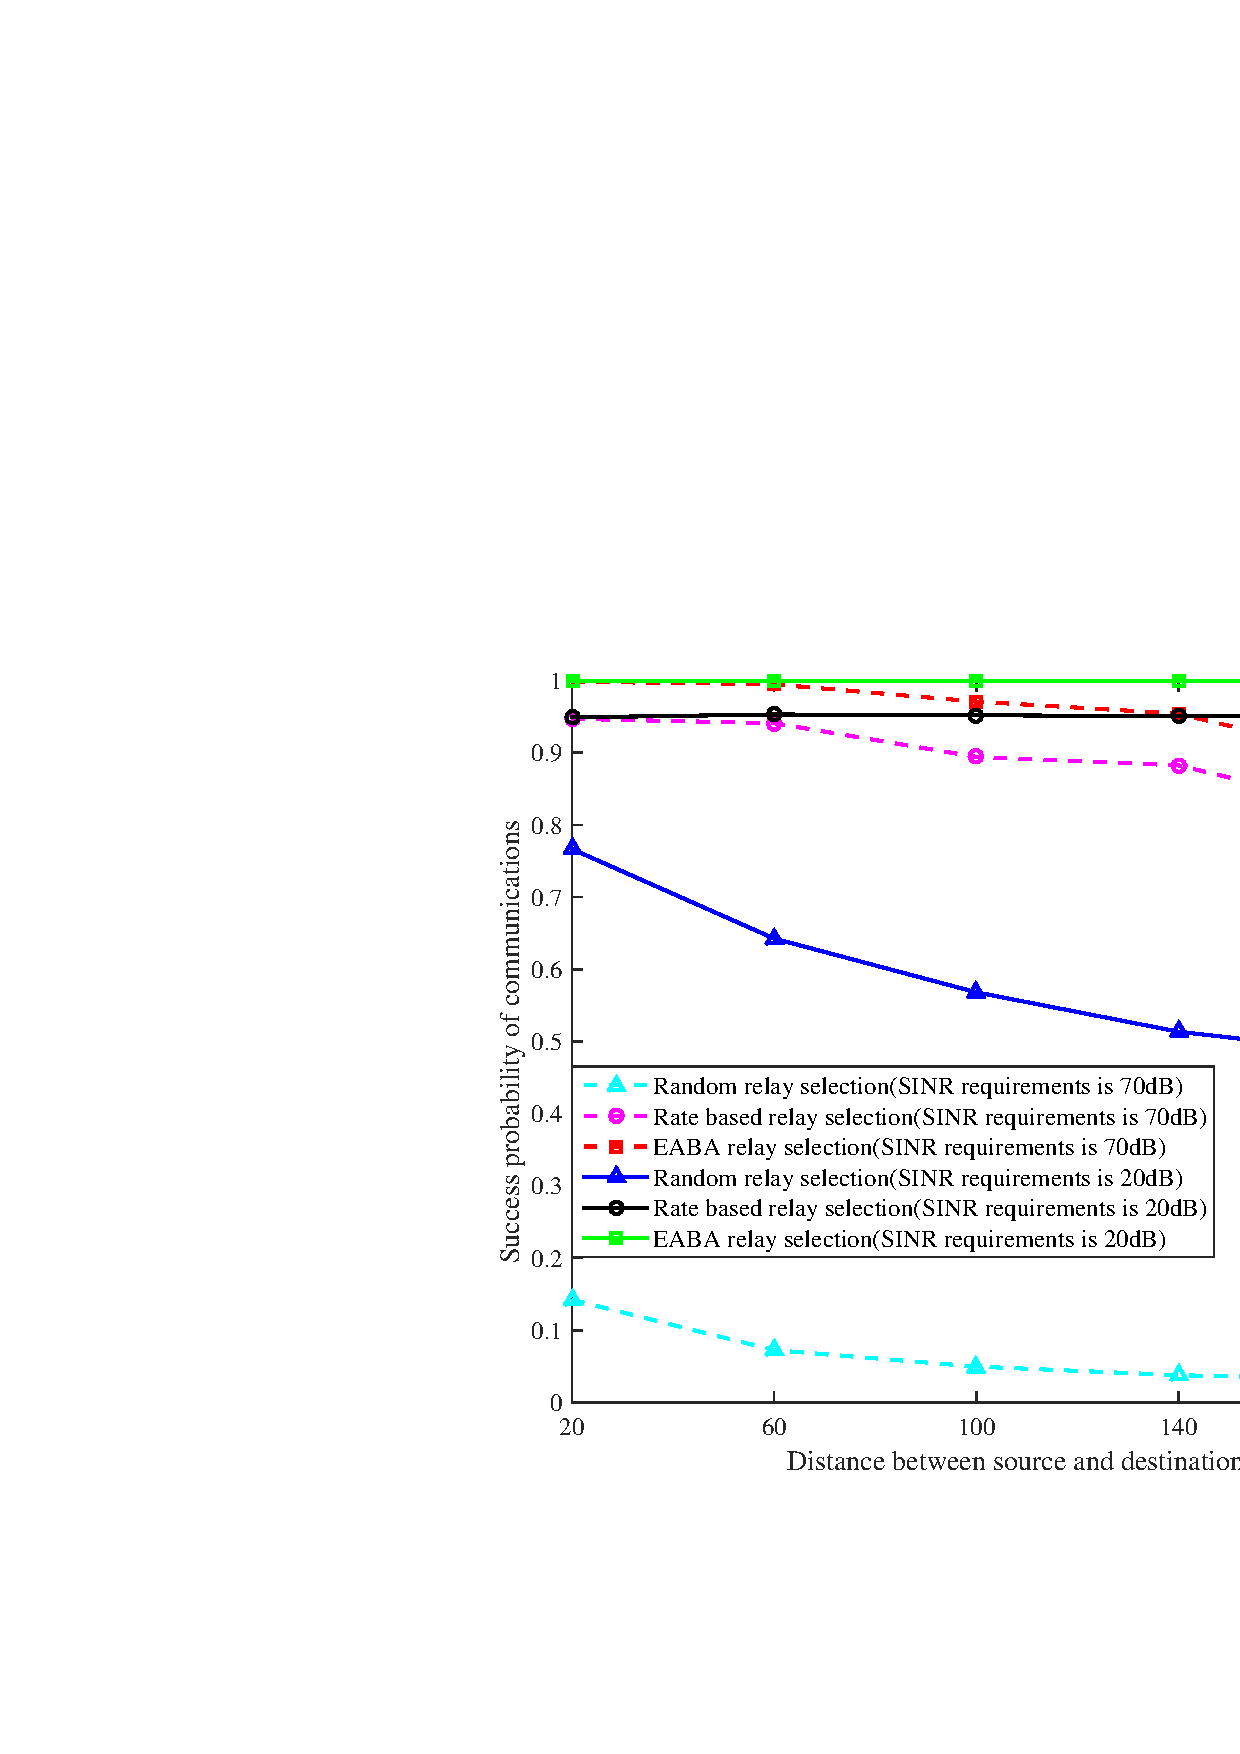
\includegraphics[width=3.5in]{fig3.pdf}
%where an .eps filename suffix will be assumed under latex,
% and a .pdf suffix will be assumed for pdflatex; or what has been declared
% via \DeclareGraphicsExtensions.
\caption{The probability of successful communications using the three relay selection methods. The RUD buffer size is 5, the uplink channel bandwidth is 720 kHz.}
\label{fig_success}
\end{figure}
%Fig4
\begin{figure}[!t]
\center
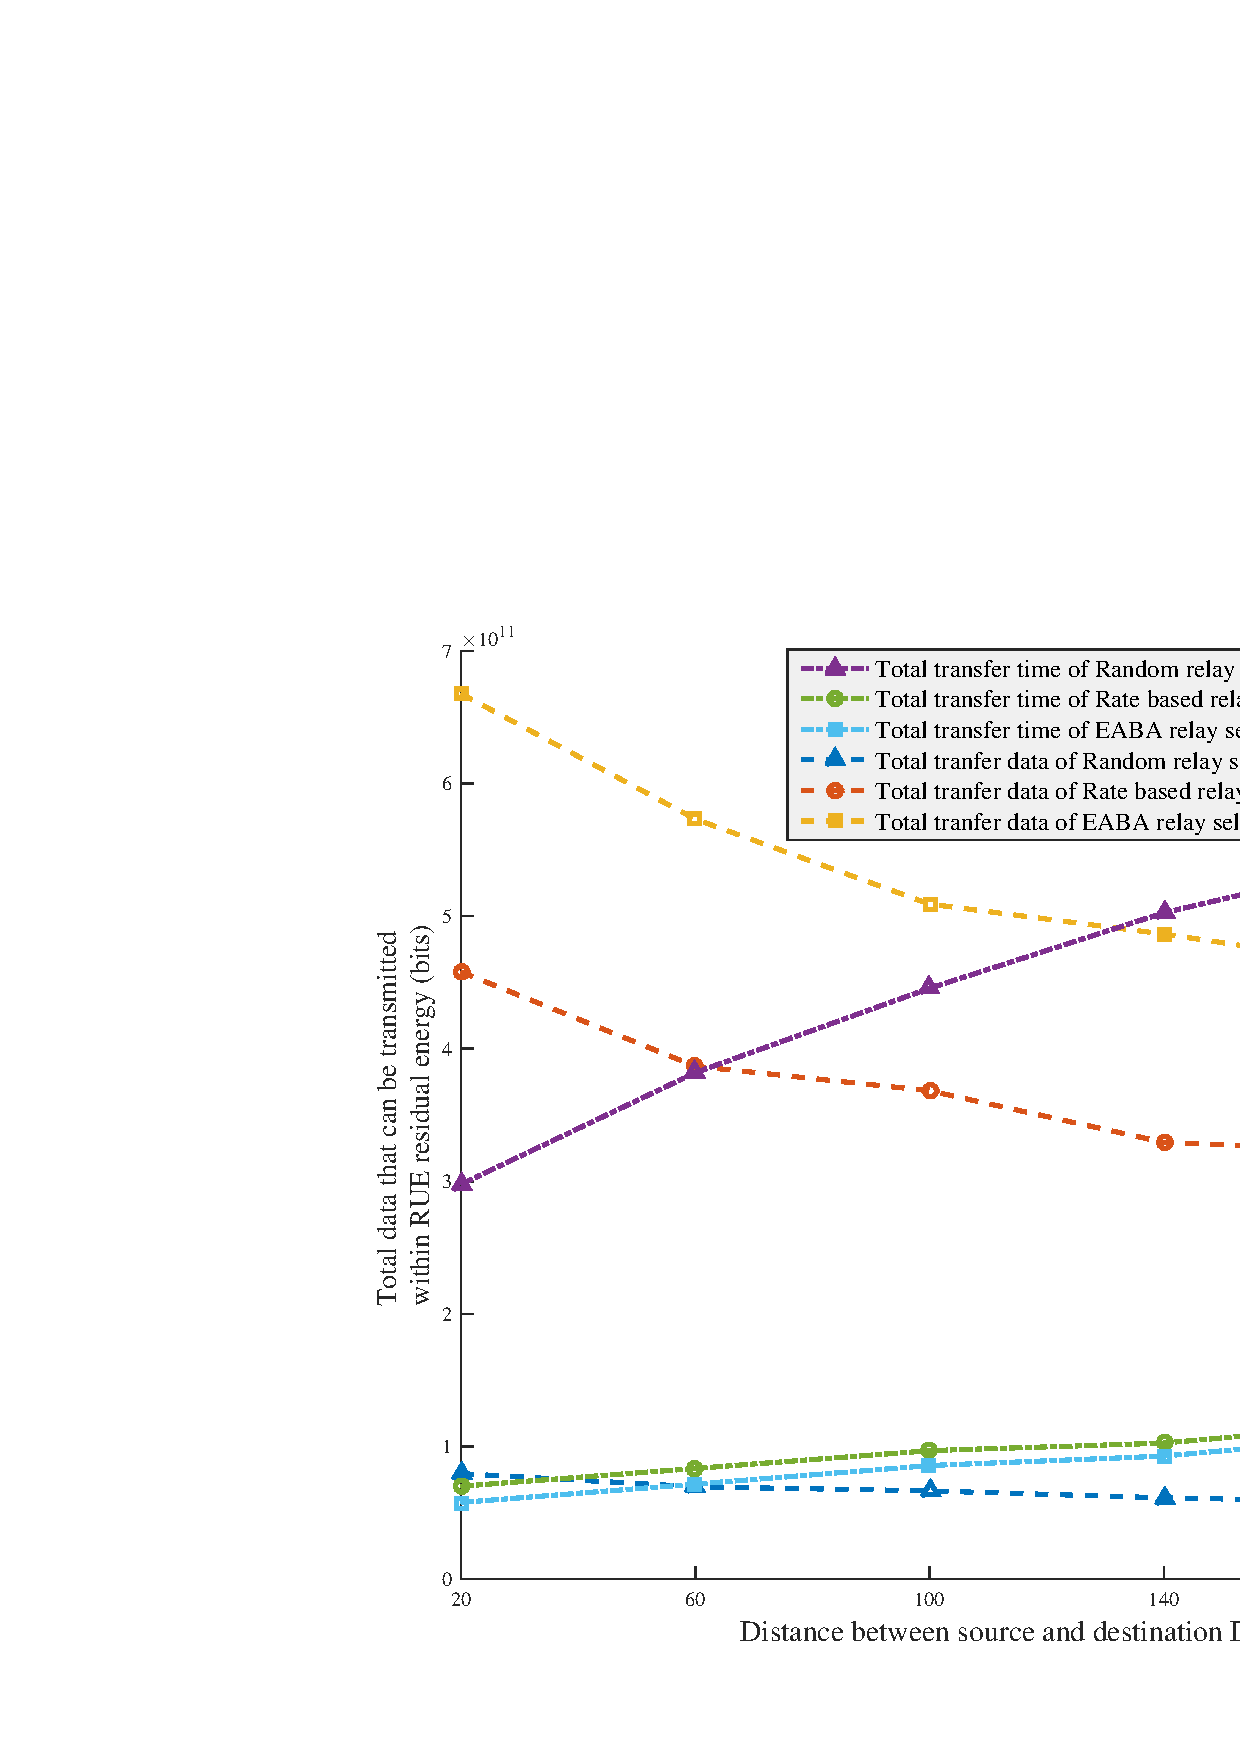
\includegraphics[width=3.5in]{fig4.pdf}
%where an .eps filename suffix will be assumed under latex,
% and a .pdf suffix will be assumed for pdflatex; or what has been declared
% via \DeclareGraphicsExtensions.
\caption{The total data transmission time and the total amount of data transmitted with three relay selection methods. The RUD buffer size is 5, the uplink channel bandwidth is 720 kHz.}
\label{fig_time}
\end{figure}

Fig. 3 demonstrates the probability of successful communications using the three relay selection methods. As the distance between DUDs $S$ and $D$ decreases, the chances of successful communication are greatly improved. The result is very plausible, as the average distance between random distributed RUDs and DUDs will decrease with the decreasing distance between the $S$ and $D$. So the channel gain of link between DUDs and RUDs will increase with an decreasing distance, which will improve the success probability of D2D communication. Specifically, the EABA relay selection presents the best performance. The reason is that random relay selection method randomly selects a link, SINR of which may not meet the requirements for D2D links and subsequently lead to communication failure. And rate based relay selection method selects a link has maximum link data rate, but the RUDs buffer states and residual energies are not considered. So the method to select a link from $S$ to RUD with maximum link data rate, but the RUD does not have enough buffer space or residual energy which may lead to communication failure. Furthermore, no matter which method is applied, D2D communication achieves higher success probability under a lower link SINR requirement.

Fig. 4 shows that the total data transmission time of the three relay selection methods become worse as the distance between $S$ and $D$ is expanded. Due to the fact that the transmission rate of both $S$-to-RUD and RUD-to-$D$ links will be reduced by expanding separation distance, directly leading to a decreased data transmission in both of the links. Thus, the total data transmission time will go up. In the three methods, the EABA method has the minimum total transmission time, because it has a higher data rate and communications success probability. The random relay selection method shows the worst performance, due to its lowest link data rate and communications success probability. Although rate based relay selection method select the fastest link, but the lower communication success probability leading to an higher transmission time than EABA method .
%Fig5
\begin{figure}[!t]
\center
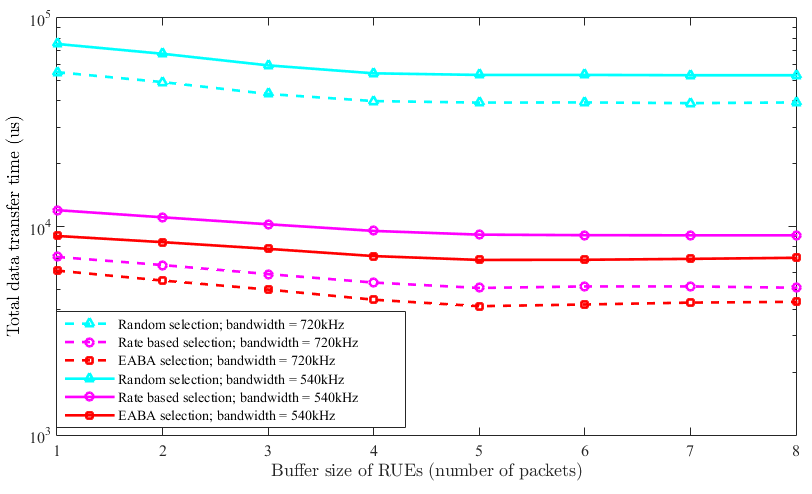
\includegraphics[width=3.5in]{fig5.pdf}
%where an .eps filename suffix will be assumed under latex,
% and a .pdf suffix will be assumed for pdflatex; or what has been declared
% via \DeclareGraphicsExtensions.
\caption{The total data transmission time with varying buffer size, and different relay selection method and channel bandwidths, where the distance between the $S$ and $D$ is 180m.}
\label{fig_time}
\end{figure}

Fig. 4 shows that the influences of the distances between the $S$ and $D$ on the total amount of data transmitted with the three relay selection methods. As the distances increasing, the path loss will significantly enhance, leading to a decreasing link transmission rate. In addition, with the same system parameters, the random method affords a much worse performance than the other two selection methods, because that the selected link data rate and residual energy of RUD is neglected in the random relay selection. Despite rate based method chooses the link which has highest transmission rate to transmit data , it will consume all of the energy of the system quickly, due to the fact that residual energy of RUD is not considered in the relay selection, leading to a smaller amount of data transmitted than EABA method. The EABA method provides the best performance, because it not only ensure the system work more time, but also ensure the link data rate.

Fig. 5 illustrates the effects of the size of RUD's buffer on the total data transmission time with the three relay selection strategies and various channel bandwidths. When we specify a bandwidth and a relay selection method, if buffer size is less than 5, increasing the buffer size of RUDs leads to a decrease in the total data transmission time. As the buffer size increases, the probability of successful communications increases, and this leads to lower total data transmission time. Otherwise, the total time isn't influenced by buffer size when it is greater than 5. The reason is that the communication failure caused due to RUDs lack of buffer size which does not happen when RUDs has enough buffer size. No matter which method is used, enhancing channel bandwidth will significantly decrease the total data transmission time, causing a bigger bandwidth leads to a higher transmisson rata for each link. In addition, with the same buffer size and channel bandwidth, the total data transmission time of EABA method is shorter than that of the random and rate based method, and the advantage becomes more dramatically when the bandwidth is comparatively small.

\section{Conclusion}
In this paper, we proposed an efficient relay selection method for Relay-Aided D2D communication in cellular network. Under the assumptions that were mentioned earlier,  we designed an Energy-Aware and Buffer-Assisted (EABA) relay selection method that jointly considered transmission rate, RUDs residual energies, and RUDs buffer states. We also described the compute processes of the transmission rate, RUDs residual energies, and RUDs buffer states. Specially, we established a relay selection method which select the best link instead of selecting best relay. Simulation results showed that the proposed method provides the best overall transmission performance compared with other relay selection methods.

\section*{Acknowledgment}
This work was supported by the National Key Technology R\&D Program (No.2015BAI01B14) and the Fundamental Research Funds for the Central Universities.
% references section
% trigger a \newpage just before the given reference
% number - used to balance the columns on the last page
% adjust value as needed - may need to be readjusted if
% the document is modified later
\bibliographystyle{IEEEtran}
\bibliography{ref}

\end{document} 